\begin{frame}{privacy and permissions}
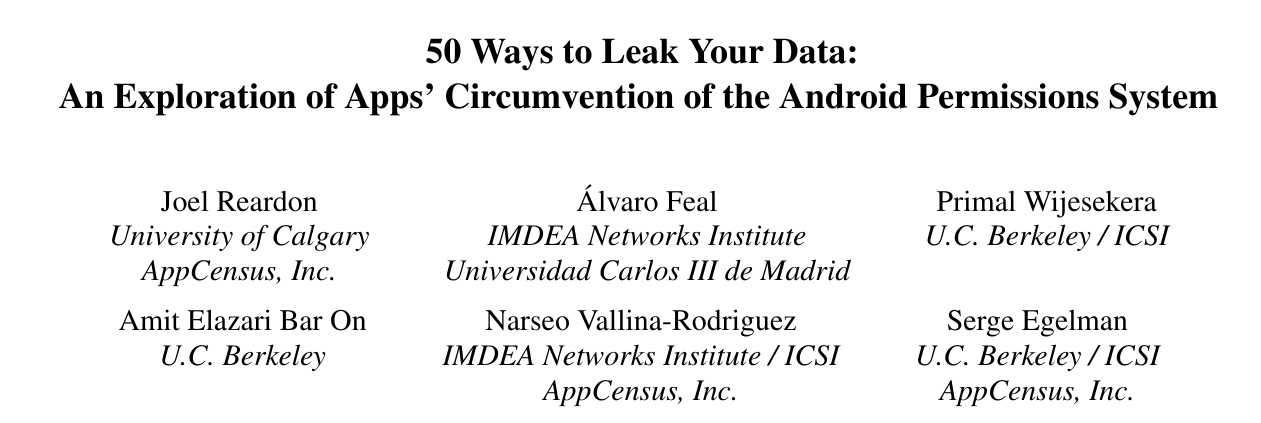
\includegraphics[width=0.7\textwidth]{../sandbox/priv-and-perm}
    \begin{itemize}
    \item 2019 paper
    \item many mobile application permissions related to privacy
    \item getting phone ID, email address, location, \ldots
    \item but applications (especially ad libraries) find workarounds
    \end{itemize}
\end{frame}

\begin{frame}{permissions being insufficient}
    \begin{itemize}
    \item permissions check limited API calls for getting private info,\ldots
    \item \ldots but there were alternative, unfiltered system calls for
    \vspace{.5cm}
    \item getting MAC address (effectively phone ID)
        \begin{itemize}
        \item Linux \texttt{ioctl} system call on socket
        \end{itemize}
    \item WiFi base station address
        \begin{itemize}
        \item ARP cache (recently seen machines on network, to know where to send packets)
        \end{itemize}
    \item location
        \begin{itemize}
        \item geolocation tag on recent photos
        \end{itemize}
    \end{itemize}
\end{frame}

\begin{frame}{covert channels}
    \begin{itemize}
    \item advertising libraries would store phone ID/account info in a file
        \begin{itemize}
        \item \ldots when they had permissions to retrieve it
        \end{itemize}
    \item and would read phone ID/account info from a file
        \begin{itemize}
        \item \ldots when they did not
        \end{itemize}
    \end{itemize}
\end{frame}
